\documentclass[aspectratio=169, 10pt]{beamer}

% =========================================================================
% MINIMALIST BEIGE & NAVY THEME (MARP / PROJECT PROPOSAL STYLE)
% Custom crafted to match the user's visual identity:
% Background: #F3EBE1 (Warm Cream Beige)
% Typography & Elements: #262E5B (Deep Indigo Navy)
% Signature: Right-edge vertical Navy bar with rounded inner corners
% =========================================================================

\usetheme{default}
\setbeamertemplate{navigation symbols}{}
\setbeamertemplate{headline}{}
\setbeamertemplate{footline}{}

\usepackage{fontspec}
% [SỬA LỖI 1] Segoe UI chỉ có trên Windows -> máy khác/Overleaf báo "font not found".
% Tự động dùng font dự phòng nếu không có Segoe UI.
\IfFontExistsTF{Segoe UI}{\setsansfont{Segoe UI}\setmainfont{Segoe UI}}{%
  \IfFontExistsTF{Carlito}{\setsansfont{Carlito}\setmainfont{Carlito}}{%
    \setsansfont{DejaVu Sans Condensed}\setmainfont{DejaVu Sans Condensed}}}

\usepackage{graphicx}
\usepackage{booktabs}
\usepackage{amsmath,amssymb}
\usepackage{xcolor}
\usepackage{tikz}
\usetikzlibrary{calc,positioning,shapes.geometric,arrows.meta}

% --- COLOR DEFINITIONS ---
\definecolor{bgBeige}{RGB}{243, 235, 225}    % #F3EBE1 - Warm Beige Canvas
\definecolor{navyMain}{RGB}{38, 46, 91}      % #262E5B - Deep Indigo Navy
\definecolor{navyMuted}{RGB}{85, 95, 140}    % Muted Navy for subtext/metadata
\definecolor{navyLight}{RGB}{228, 225, 235}  % Soft tinted fill
\definecolor{accentDark}{RGB}{185, 28, 28}   % Alert crimson

\setbeamercolor{background canvas}{bg=bgBeige}
\setbeamercolor{normal text}{fg=navyMain}
\setbeamercolor{structure}{fg=navyMain}

% Set margins so text never touches the right navy bar
\setbeamersize{text margin left=1.0cm, text margin right=1.8cm}

% --- SIGNATURE BACKGROUND WITH RIGHT NAVY ACCENT BAR ---
\setbeamertemplate{background}{
    \begin{tikzpicture}[remember picture,overlay]
        % Base Beige Canvas
        \fill[bgBeige] (current page.south west) rectangle (current page.north east);
        % Right vertical navy bar with 2 rounded inside corners (top-left & bottom-left)
        \fill[navyMain, rounded corners=16pt] 
            ($(current page.north east)+(-1.05cm, 0)$) rectangle ($(current page.south east)+(1.0cm, 0)$);
    \end{tikzpicture}
}

% --- CUSTOM SLIDE HEADER ---
\newcommand{\slideheader}[2]{%
    \vspace*{-0.15cm}%
    {\fontsize{7.5pt}{9pt}\selectfont \textbf{\color{navyMuted}\MakeUppercase{#1}}}\\[0.03cm]
    {\fontsize{13.5pt}{16pt}\selectfont \textbf{\color{navyMain}\MakeUppercase{#2}}}\\[0.08cm]
}

% --- CUSTOM FOOTER NUMBER ---
\newcommand{\slidenumber}[1]{%
    \begin{tikzpicture}[remember picture,overlay]
        \node[anchor=south east] at ($(current page.south east)+(-1.4cm, 0.35cm)$) {
            \textcolor{navyMuted}{\fontsize{8.5pt}{10pt}\selectfont \textbf{\insertframenumber}}
        };
        \node[anchor=south west] at ($(current page.south west)+(1.0cm, 0.35cm)$) {
            \textcolor{navyMuted}{\fontsize{7pt}{8pt}\selectfont \textit{Hands-On Data Visualization} -- Jack Dougherty \& Ilya Ilyankou}
        };
    \end{tikzpicture}%
}

% --- PILL BOX MACRO ---

\definecolor{boxBg}{RGB}{230, 221, 208}      % Tinted card bg #E6DDD0
\definecolor{accentRed}{RGB}{185, 28, 28}    % Alert crimson #B91C1C

\newcommand{\calloutbox}[3][\textwidth]{%
    \begin{tikzpicture}
        \node[
            fill=boxBg,
            draw=navyMain,
            line width=0.8pt,
            rounded corners=4pt,
            inner sep=5pt,
            text width=#1-14pt,
            align=left
        ] {
            {\fontsize{8.5pt}{10.5pt}\selectfont \textbf{\color{navyMain}#2}}\\[0.03cm]
            {\fontsize{7.5pt}{9.5pt}\selectfont \color{navyMain}#3}
        };
    \end{tikzpicture}%
}

\newcommand{\pillbox}[2][]{%
    \begin{tikzpicture}
        \node[
            draw=navyMain,
            rounded corners=10pt,
            line width=1.1pt,
            inner xsep=12pt,
            inner ysep=4pt,
            text=navyMain,
            #1
        ] {\textbf{#2}};
    \end{tikzpicture}%
}

% [SỬA LỖI 2] Thiếu file ảnh trong images/ -> lỗi "File not found" và dừng biên dịch.
% Nếu ảnh có thật: chèn bình thường. Nếu chưa có: vẽ khung giữ chỗ cùng kích thước.
\pgfkeys{/ph/.is family, /ph,
  width/.store in=\phw, height/.store in=\phh, .unknown/.code={}}
\let\origincludegraphics\includegraphics
\renewcommand{\includegraphics}[2][]{%
  \IfFileExists{#2}{\origincludegraphics[#1]{#2}}{%
    \begingroup
    \pgfkeys{/ph, width=\linewidth, height=0.4\textheight, #1}%
    \begin{tikzpicture}
      \node[draw=navyMuted, dashed, line width=0.7pt, fill=white!55!bgBeige, rounded corners=3pt,
            minimum width=\phw, minimum height={0.8*(\phh)}, text width={\phw-8pt}, align=center,
            font=\fontsize{6pt}{7.5pt}\selectfont, text=navyMuted]
        {\textbf{[Chèn ảnh]}\\\detokenize{#2}};
    \end{tikzpicture}%
    \endgroup}}

\begin{document}


\begin{frame}[plain, c]


\begin{tikzpicture}[remember picture,overlay]
    \node[anchor=north west] at ($(current page.north west)+(1.0cm, -0.8cm)$) {
        \textcolor{navyMuted}{\fontsize{8.5pt}{10.5pt}\selectfont Tháng 10, 2026}
    };
    \node[anchor=west, text width=0.76\textwidth] at ($(current page.west)+(1.0cm, 0.3cm)$) {
        {\fontsize{13pt}{15pt}\selectfont \textbf{\color{navyMuted} PHẦN 3 • BÁO CÁO CHUYÊN ĐỀ}}\\[0.25cm]
        {\fontsize{28pt}{32pt}\selectfont \textbf{\color{navyMain} TRỰC QUAN HÓA KHÔNG GIAN}}\\[0.12cm]
        {\fontsize{20pt}{24pt}\selectfont \textbf{\color{navyMain} MAP YOUR DATA}}\\[0.35cm]
        \pillbox{\fontsize{9.5pt}{11.5pt}\selectfont Tư Duy Thiết Kế Bản Đồ \& Phân Tích Dữ Liệu Địa Lý (Chương 7)}\\[0.45cm]
        {\fontsize{8.5pt}{10.5pt}\selectfont \color{navyMuted} Thuyết trình: \textbf{Người 3} • Tác phẩm: \textit{Hands-On Data Visualization} (Jack Dougherty \& Ilya Ilyankou)}
    };
\end{tikzpicture}
\slidenumber{01}
\end{frame}

% ==================== SLIDE 2: MỤC LỤC PHẦN 3 ====================


\begin{frame}[plain, t]


\slideheader{Phần 3 • Tổng Quan}{Nội Dung Trình Bày (Our Contents)}
\begin{columns}[T]
\begin{column}{0.31\textwidth}
\begin{tikzpicture}
    \node[draw=navyMain, fill=boxBg, rounded corners=6pt, line width=0.9pt, inner sep=7pt, text width=\textwidth-16pt, align=left] {
        {\fontsize{9.5pt}{11.5pt}\selectfont \textbf{\color{navyMain} 01. BẢN CHẤT DỮ LIỆU}}\\[0.05cm]
        {\fontsize{8pt}{9.5pt}\selectfont \textbf{\color{navyMuted} Không Gian \& Giải Phẫu}}\\[0.15cm]
        {\fontsize{7.2pt}{9pt}\selectfont \color{navyMain}
        • Khi nào nên/không nên vẽ\\
        • Lớp nền Raster vs. Vector\\
        • 3 hình học: Point, Line, Polygon\\
        • Phân biệt Point vs Polygon\\
        • 6 loại bản đồ thông dụng}
    };
\end{tikzpicture}
\end{column}
\begin{column}{0.31\textwidth}
\begin{tikzpicture}
    \node[draw=navyMain, fill=boxBg, rounded corners=6pt, line width=0.9pt, inner sep=7pt, text width=\textwidth-16pt, align=left] {
        {\fontsize{9.5pt}{11.5pt}\selectfont \textbf{\color{navyMain} 02. NGUYÊN LÝ THỰC CHIẾN}}\\[0.05cm]
        {\fontsize{8pt}{9.5pt}\selectfont \textbf{\color{navyMuted} Thiết Kế Bản Đồ}}\\[0.15cm]
        {\fontsize{7.2pt}{9pt}\selectfont \color{navyMain}
        • Quy tắc 1: Chỉ biểu diễn 1 biến\\
        • Tránh quá tải khi chồng 2 biến\\
        • Dùng Scatter Chart thay thế\\
        • Quy tắc 2: Chọn đơn vị nhỏ hơn\\
        • Bài toán diện tích MAUP}
    };
\end{tikzpicture}
\end{column}
\begin{column}{0.31\textwidth}
\begin{tikzpicture}
    \node[draw=navyMain, fill=boxBg, rounded corners=6pt, line width=0.9pt, inner sep=7pt, text width=\textwidth-16pt, align=left] {
        {\fontsize{9.5pt}{11.5pt}\selectfont \textbf{\color{navyMain} 03. CHOROPLETH \& CHUẨN HÓA}}\\[0.05cm]
        {\fontsize{8pt}{9.5pt}\selectfont \textbf{\color{navyMuted} Màu Sắc \& Nội Suy}}\\[0.15cm]
        {\fontsize{7.2pt}{9pt}\selectfont \color{navyMain}
        • Bảng màu ColorBrewer chuẩn\\
        • Bậc thang (Steps) vs. Liên tục\\
        • 3 nội suy: Linear, Quantile, Jenks\\
        • Bắt buộc chuẩn hóa (Covid-19)\\
        • Bản đồ thời gian thực \& Null Island}
    };
\end{tikzpicture}
\end{column}
\end{columns}
\slidenumber{02}
\end{frame}

% ==================== SLIDE 3: CHUYỂN TIẾP MỤC 01 ====================


\begin{frame}[plain, c]


\begin{tikzpicture}[remember picture,overlay]
    \node[anchor=west, text width=0.76\textwidth] at ($(current page.west)+(1.0cm, 0.2cm)$) {
        {\fontsize{13pt}{15pt}\selectfont \textbf{\color{navyMuted} PHẦN 3 • MỤC 01}}\\[0.25cm]
        {\fontsize{28pt}{32pt}\selectfont \textbf{\color{navyMain} BẢN CHẤT DỮ LIỆU}}\\[0.12cm]
        {\fontsize{22pt}{26pt}\selectfont \textbf{\color{navyMain} KHÔNG GIAN}}\\[0.35cm]
        \pillbox{\fontsize{10pt}{12pt}\selectfont Deconstructing a Map \& Spatial Data Types}\\[0.45cm]
        {\normalsize \color{navyMuted} \textit{``Chỉ vì dữ liệu có yếu tố địa lý\\không có nghĩa là bạn bắt buộc phải vẽ bản đồ.''}}
    };
\end{tikzpicture}
\slidenumber{03}
\end{frame}

% ==================== SLIDE 4: KHI NÀO NÊN (VÀ KHÔNG NÊN) VẼ BẢN ĐỒ? ====================


\begin{frame}[plain, t]


\slideheader{Mục 01 • Bản Chất Không Gian}{Khi Nào Nên (Và Không Nên) Vẽ Bản Đồ?}
\begin{columns}[T]
\begin{column}{0.52\textwidth}
{\fontsize{8.2pt}{10.5pt}\selectfont
\calloutbox[\textwidth]{Câu Hỏi Cốt Lõi Trước Khi Vẽ Bản Đồ}{
    \textit{``Vị trí địa lý và quy luật phân bố không gian (spatial pattern) có thực sự quan trọng đối với câu chuyện của bạn không?''}
}

\vspace{0.12cm}
\textbf{Khi nào Bản đồ là lựa chọn tối ưu?}
\begin{itemize}\setlength{\itemsep}{1.5pt}
    \item Khi người xem cần thấy \textbf{khoảng cách tương đối} giữa các điểm.
    \item Khi muốn nhận diện \textbf{sự tập trung theo cụm (clusters)}.
    \item Khi phân tích \textbf{xu hướng lan tỏa theo vùng} (tâm dịch bệnh, vùng ngập lụt, phân hóa kinh tế Đông -- Tây).
\end{itemize}
}
\end{column}
\begin{column}{0.44\textwidth}
\calloutbox[\textwidth]{Khi Nào Biểu Đồ Thường (Chart) Kể Chuyện Tốt Hơn?}{
    • \textbf{So sánh thứ hạng cao thấp:} Biểu đồ thanh ngang (\textbf{Bar Chart}) chính xác hơn nhiều vì mắt người so sánh chiều dài tốt hơn diện tích vùng.\\
    • \textbf{Tốc độ biến động theo thời gian:} Biểu đồ đường (\textbf{Line Chart}) thể hiện xu hướng dốc rõ hơn chuỗi bản đồ.\\
    • \textbf{Mối quan hệ giữa 2 biến số:} Biểu đồ phân tán (\textbf{Scatter Chart}) cho thấy tương quan trực diện mà bản đồ không thể làm được!
}
\end{column}
\end{columns}
\slidenumber{04}
\end{frame}

% ==================== SLIDE 5: LỚP NỀN RASTER VS. VECTOR ====================


\begin{frame}[plain, t]


\slideheader{Mục 01 • Bản Chất Không Gian}{Giải Phẫu Bản Đồ: Lớp Nền Raster vs. Vector}
\begin{columns}[T]
\begin{column}{0.52\textwidth}
{\fontsize{7.8pt}{9.8pt}\selectfont
Bản đồ tương tác gồm: \textbf{Lớp nền (Basemap)} và \textbf{Lớp dữ liệu (Data layers)}:

\vspace{0.1cm}
\begin{table}[h]
\centering
\begin{tabular}{p{0.45\textwidth} p{0.45\textwidth}}
\toprule
\textbf{\color{navyMain} Bản đồ nền Raster} & \textbf{\color{navyMain} Bản đồ nền Vector} \\
\midrule
Ảnh chụp vệ tinh / máy bay ghép lại theo ô lưới (\textit{aerial photos}). & Dựng từ tọa độ toán học (đường xá, tòa nhà, sông ngòi). \\
\midrule
\textcolor{accentRed}{\textbf{Khi phóng to (Zoom in):}} Bị giới hạn độ phân giải ảnh gốc; \textbf{càng phóng to càng vỡ hạt và mờ nhòe (fuzzy)}. & \textbf{Khi phóng to (Zoom in):} Tái tính toán theo tỷ lệ; \textbf{giữ nguyên độ sắc nét tuyệt đối} ở mọi cấp độ thu phóng! \\
\bottomrule
\end{tabular}
\end{table}
}
\end{column}
\begin{column}{0.44\textwidth}
\centering
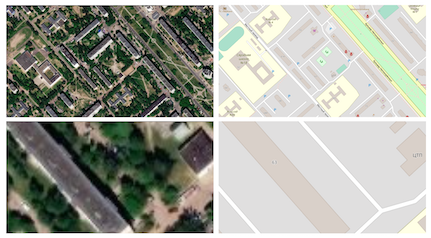
\includegraphics[width=\textwidth, height=0.52\textheight, keepaspectratio]{images/fig_7_1_raster_vs_vector.png}\\[0.15cm]
{\fontsize{6.8pt}{8pt}\selectfont \textcolor{navyMuted}{\textit{Hình 7.1: Nền Raster vệ tinh bị vỡ hạt (trái) vs Nền Vector OSM sắc nét (phải).}}}
\end{column}
\end{columns}
\slidenumber{05}
\end{frame}

% ==================== SLIDE 6: 3 KIỂU HÌNH HỌC KHÔNG GIAN ====================


\begin{frame}[plain, t]


\slideheader{Mục 01 • Bản Chất Không Gian}{3 Kiểu Hình Học Không Gian \& Cấu Trúc Bản Đồ}
\begin{columns}[T]
\begin{column}{0.52\textwidth}
{\fontsize{8.2pt}{10.5pt}\selectfont
Lớp dữ liệu phủ trên bản đồ nền gồm 3 thực thể (kinh độ, vĩ độ):

\vspace{0.12cm}
\textbf{1. Điểm (Point):}
\begin{itemize}\setlength{\itemsep}{1.5pt}
    \item Một vị trí cụ thể duy nhất $(x, y)$. VD: Tượng Nữ thần Tự do $(40.69, -74.04)$.
\end{itemize}

\textbf{2. Đa tuyến (Polyline):}
\begin{itemize}\setlength{\itemsep}{1.5pt}
    \item Chuỗi điểm liên tiếp tạo tuyến đường sắt, sông, xe buýt.
\end{itemize}

\textbf{3. Đa giác (Polygon):}
\begin{itemize}\setlength{\itemsep}{1.5pt}
    \item Đoạn thẳng khép kín bao quanh ranh giới (Tract, Hạt, Bang).
\end{itemize}

\vspace{0.12cm}
\textbf{Thành phần bổ trợ bắt buộc:} Tiêu đề, Chú giải (Legend), Nút zoom, Thước tỷ lệ (Scale), Mũi tên Bắc, Popup/Tooltip và Nguồn.
}
\end{column}
\begin{column}{0.44\textwidth}
\centering
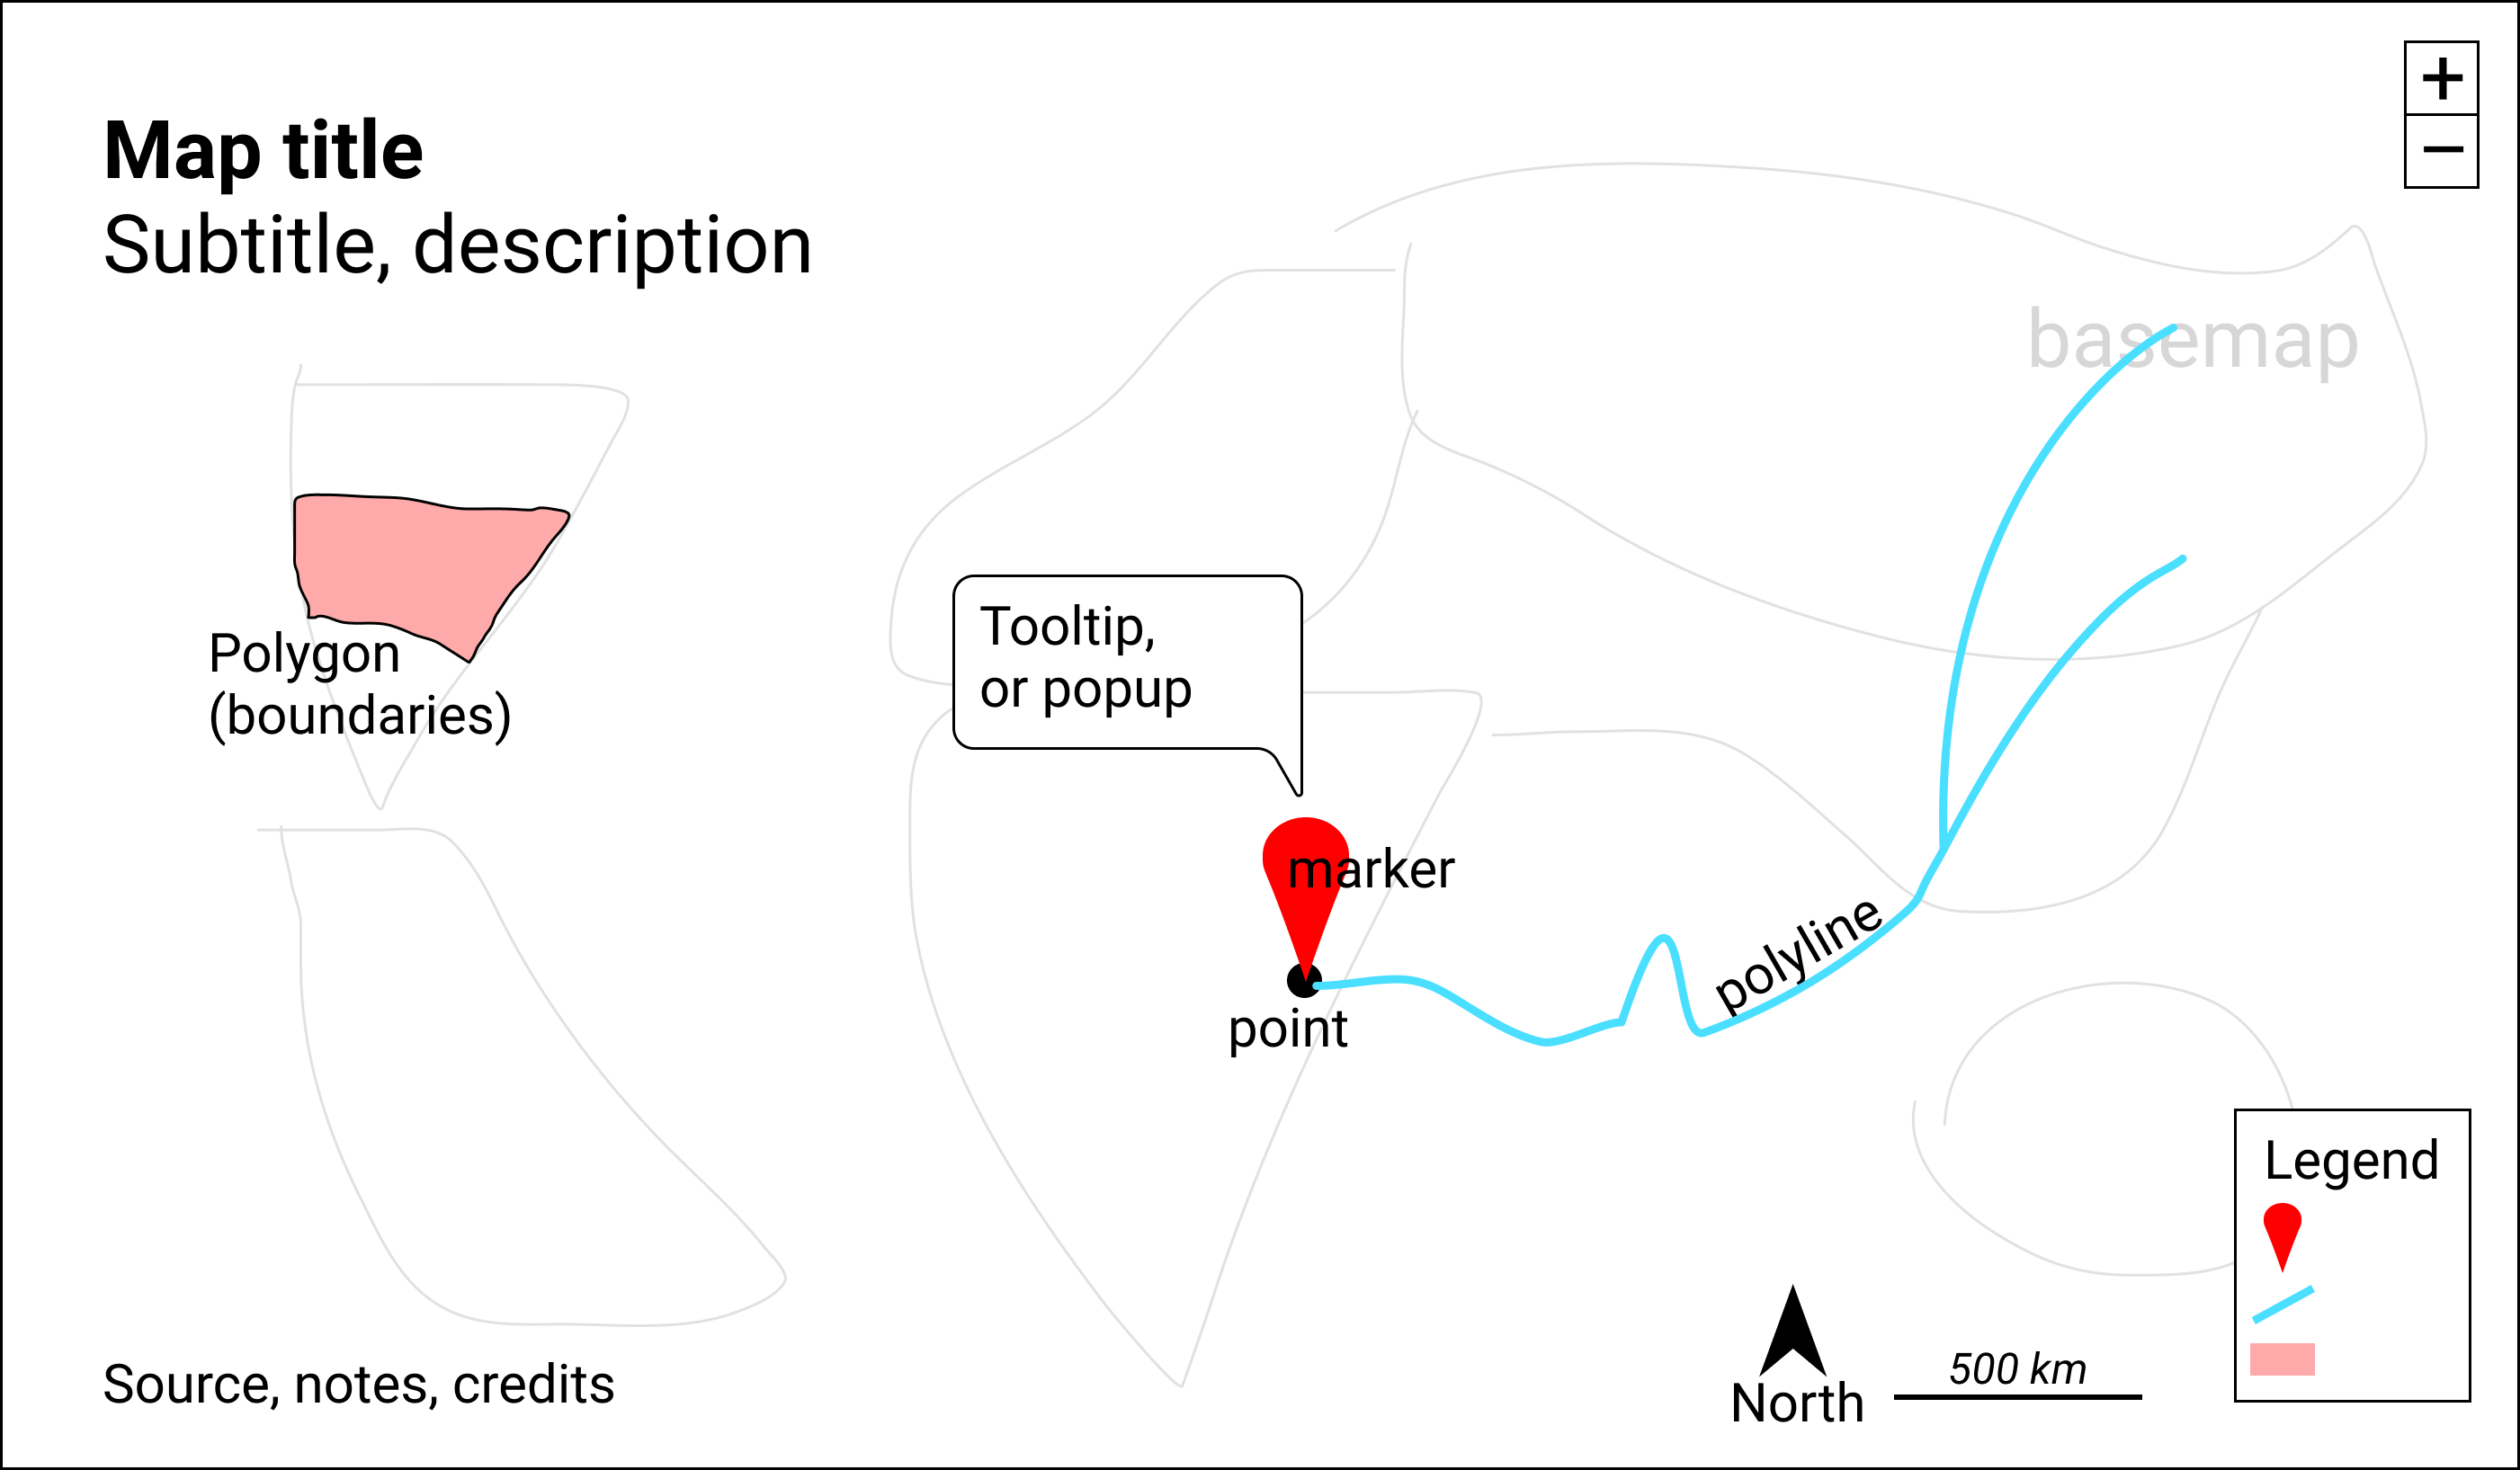
\includegraphics[width=\textwidth, height=0.52\textheight, keepaspectratio]{images/fig_7_2_map_elements.png}\\[0.15cm]
{\fontsize{6.8pt}{8pt}\selectfont \textcolor{navyMuted}{\textit{Hình 7.2: Giải phẫu các thành phần của một bản đồ tương tác chuẩn.}}}
\end{column}
\end{columns}
\slidenumber{06}
\end{frame}

% ==================== SLIDE 7: PHÂN BIỆT POINT VS. POLYGON ====================


\begin{frame}[plain, t]


\slideheader{Mục 01 • Bản Chất Không Gian}{Phân Biệt Dữ Liệu Điểm (Point) vs. Vùng (Polygon)}
\begin{columns}[T]
\begin{column}{0.52\textwidth}
{\fontsize{7.8pt}{9.8pt}\selectfont
\begin{table}[h]
\centering
\begin{tabular}{p{0.55\textwidth} p{0.35\textwidth}}
\toprule
\textbf{\color{navyMain} Dữ liệu địa lý (California)} & \textbf{\color{navyMain} Bản chất \& Biểu diễn} \\
\midrule
• Tọa độ \texttt{36.48, -118.56}\newline • Địa chỉ \texttt{2800 E Observatory Rd}\newline • Ngã tư \texttt{Haight \& Ashbury St}\newline • Công viên \texttt{Balboa Park} & \textbf{POINT (Điểm)}\newline $\rightarrow$ Vẽ Bản đồ Điểm (\textit{Point / Symbol Map}) \\
\midrule
• Khu điều tra \texttt{Census tract 4087}\newline • Thành phố \texttt{City of Los Angeles}\newline • Hạt \texttt{San Diego County}\newline • Tiểu bang \texttt{State of California} & \textbf{POLYGON (Vùng)}\newline $\rightarrow$ Vẽ Bản đồ Phân vùng màu (\textit{Choropleth Map}) \\
\bottomrule
\end{tabular}
\end{table}
}
\end{column}
\begin{column}{0.44\textwidth}
\calloutbox[\textwidth]{3 Ngoại Lệ Linh Hoạt Tùy Theo Câu Chuyện}{
    1. \textbf{Biến Vùng thành Điểm:} Tìm tâm điểm (\textit{Centroid}) của thành phố Los Angeles để vẽ hình tròn tăng trưởng dân số.\\[0.08cm]
    2. \textbf{Biến Điểm thành Vùng:} Vẽ công viên Balboa Park thành đa giác $1,8\text{ dặm vuông}$ nếu nghiên cứu tỷ lệ đất công viên.\\[0.08cm]
    3. \textbf{Gộp Điểm thành Vùng (Pivot):} Cộng số giường bệnh của từng bệnh viện (Points) để tô màu năng lực y tế toàn Hạt (Polygon).
}
\end{column}
\end{columns}
\slidenumber{07}
\end{frame}

% ==================== SLIDE 8: HỆ SINH THÁI CÁC LOẠI BẢN ĐỒ ====================


\begin{frame}[plain, t]


\slideheader{Mục 01 • Bản Chất Không Gian}{Hệ Sinh Thái 6 Loại Bản Đồ Trực Quan Hóa}
\begin{columns}[T]
\begin{column}{0.52\textwidth}
{\fontsize{8pt}{10pt}\selectfont
\begin{itemize}\setlength{\itemsep}{2pt}
    \item \textbf{1. Point Map with Custom Icons:} Đánh dấu vị trí kèm cửa sổ Popup ảnh và chi tiết.
    \item \textbf{2. Symbol Point Map (Ký hiệu tỷ lệ):} Vòng tròn có \textbf{kích thước \& màu sắc} biến thiên theo số liệu (VD: Biến động dân số 300 thành phố Mỹ).
    \item \textbf{3. Choropleth Map (Phân vùng màu):} Tô màu các đa giác theo thang giá trị.
    \item \textbf{4. Heat Point Map (Bản đồ nhiệt):} Biểu diễn mật độ tập trung dày đặc (hotspots).
    \item \textbf{5. Story Map \& Polyline Map:} Dẫn dắt người xem theo hành trình hoặc tuyến mạng lưới.
    \item \textbf{6. Live Map (Thời gian thực):} Kết nối dữ liệu mở cập nhật hàng ngày.
\end{itemize}
}
\end{column}
\begin{column}{0.44\textwidth}
\centering
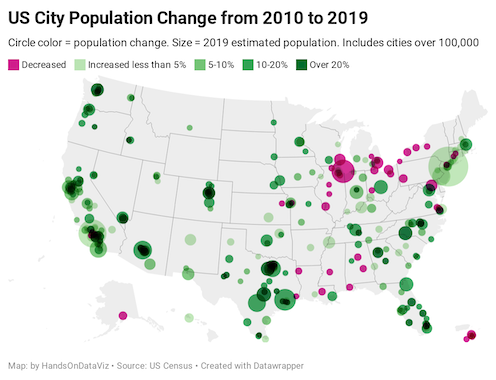
\includegraphics[width=\textwidth, height=0.52\textheight, keepaspectratio]{images/fig_7_34_symbol_map.png}\\[0.15cm]
{\fontsize{6.8pt}{8pt}\selectfont \textcolor{navyMuted}{\textit{Hình 7.34: Symbol Point Map biến động dân số 300 thành phố Mỹ 2010--2019.}}}
\end{column}
\end{columns}
\slidenumber{08}
\end{frame}

% ==================== SLIDE 9: CHUYỂN TIẾP MỤC 02 ====================


\begin{frame}[plain, c]


\begin{tikzpicture}[remember picture,overlay]
    \node[anchor=west, text width=0.76\textwidth] at ($(current page.west)+(1.0cm, 0.2cm)$) {
        {\fontsize{13pt}{15pt}\selectfont \textbf{\color{navyMuted} PHẦN 3 • MỤC 02}}\\[0.25cm]
        {\fontsize{28pt}{32pt}\selectfont \textbf{\color{navyMain} NGUYÊN LÝ THIẾT KẾ}}\\[0.12cm]
        {\fontsize{22pt}{26pt}\selectfont \textbf{\color{navyMain} BẢN ĐỒ THỰC CHIẾN}}\\[0.35cm]
        \pillbox{\fontsize{10pt}{12pt}\selectfont Core Map Design Principles}\\[0.45cm]
        {\normalsize \color{navyMuted} \textit{``Tránh quá tải thị giác và lựa chọn độ phân giải địa lý tối ưu.''}}
    };
\end{tikzpicture}
\slidenumber{09}
\end{frame}

% ==================== SLIDE 10: QUY TẮC 1: CHỈ 1 BIẾN SỐ ====================


\begin{frame}[plain, t]


\slideheader{Mục 02 • Nguyên Lý Thiết Kế}{Quy Tắc 1: Chỉ 1 Biến Số, Đừng Nhồi Nhét 2 Biến!}
\begin{columns}[T]
\begin{column}{0.52\textwidth}
{\fontsize{8.2pt}{10.5pt}\selectfont
\textbf{Sai lầm:} Chồng 2 biến khác nhau lên cùng 1 bản đồ.

\vspace{0.12cm}
\textbf{Bài toán Thu nhập \& Trình độ Đại học tại 8 quận:}
\begin{itemize}\setlength{\itemsep}{1.5pt}
    \item \textbf{(a) Choropleth xanh (Thu nhập):} Tốt (thấy vùng Tây Bắc giàu).
    \item \textbf{(b) Symbol vòng tròn cam (Học vấn):} Tốt (nhìn riêng lẻ).
    \item \textcolor{accentRed}{\textbf{[Sai] (c) Chồng (b) đè lên (a):}} Vừa tô nền vừa đè vòng tròn $\rightarrow$ \textbf{Quá tải thị giác (Overloaded)!} Mắt người không thể giải mã nổi mối liên hệ.
    \item \textbf{[Chuẩn] (d) Giải pháp chuẩn:} Dùng \textbf{Scatter Chart} để thể hiện trực diện mối tương quan 2 biến!
\end{itemize}
}
\end{column}
\begin{column}{0.44\textwidth}
\centering
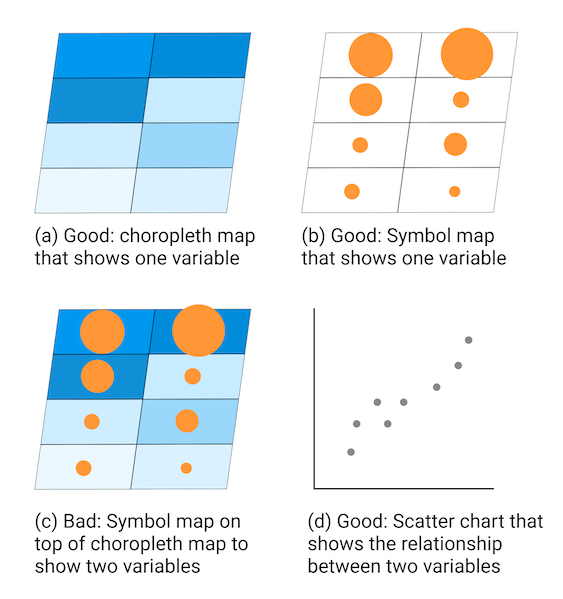
\includegraphics[width=\textwidth, height=0.52\textheight, keepaspectratio]{images/fig_7_3_one_var_not_two.png}\\[0.15cm]
{\fontsize{6.8pt}{8pt}\selectfont \textcolor{navyMuted}{\textit{Hình 7.3: (a,b) Tốt; (c) Quá tải khi chồng 2 biến; (d) Dùng Scatter chart.}}}
\end{column}
\end{columns}
\slidenumber{10}
\end{frame}

% ==================== SLIDE 11: QUY TẮC 2: CHỌN ĐƠN VỊ ĐỊA LÝ NHỎ HƠN (MAUP) ====================


\begin{frame}[plain, t]


\slideheader{Mục 02 • Nguyên Lý Thiết Kế}{Quy Tắc 2: Chọn Đơn Vị Địa Lý Nhỏ Hơn (Bài Toán MAUP)}
\begin{columns}[T]
\begin{column}{0.52\textwidth}
{\fontsize{8.2pt}{10.5pt}\selectfont
\textbf{Bài toán Đơn vị Diện tích Khả biến (MAUP):}
Cách gộp lớn hay chia nhỏ ranh giới sẽ làm thay đổi hoàn toàn nhận thức!

\vspace{0.12cm}
\textbf{Case Study Zillow: Giá nhà Đông Bắc Mỹ (9/2020):}
\begin{itemize}\setlength{\itemsep}{1.5pt}
    \item \textbf{Cấp Bang (State level - Trái):} Đơn điệu, chỉ thấy bang Massachusetts đậm hơn; \textbf{che giấu hoàn toàn sự chênh lệch nội bộ}.
    \item \textbf{Cấp Quận/Hạt (County level - Phải):} Lộ rõ các \textbf{cụm giá nhà đắt đỏ quanh New York, Long Island, Boston} so với vùng nông thôn ngay trong cùng bang!
\end{itemize}

\vspace{0.12cm}
$\rightarrow$ \textbf{Nguyên tắc:} Luôn ưu tiên cấp địa lý nhỏ hơn kèm viền bang phân định rõ.
}
\end{column}
\begin{column}{0.44\textwidth}
\centering
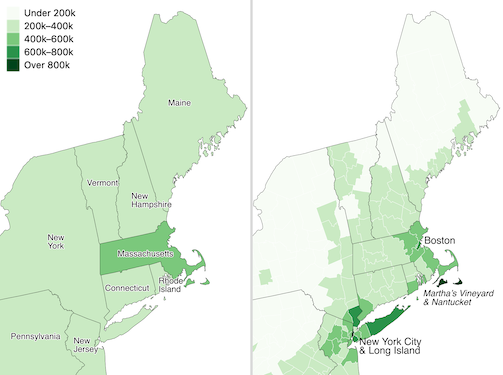
\includegraphics[width=\textwidth, height=0.52\textheight, keepaspectratio]{images/fig_7_4_state_vs_county.png}\\[0.15cm]
{\fontsize{6.8pt}{8pt}\selectfont \textcolor{navyMuted}{\textit{Hình 7.4: Giá nhà cấp Bang (trái - đơn điệu) vs cấp Quận (phải - chi tiết).}}}
\end{column}
\end{columns}
\slidenumber{11}
\end{frame}

% ==================== SLIDE 12: CHUYỂN TIẾP MỤC 03 ====================


\begin{frame}[plain, c]


\begin{tikzpicture}[remember picture,overlay]
    \node[anchor=west, text width=0.76\textwidth] at ($(current page.west)+(1.0cm, 0.2cm)$) {
        {\fontsize{13pt}{15pt}\selectfont \textbf{\color{navyMuted} PHẦN 3 • MỤC 03}}\\[0.25cm]
        {\fontsize{28pt}{32pt}\selectfont \textbf{\color{navyMain} THIẾT KẾ BẢN ĐỒ CHOROPLETH}}\\[0.12cm]
        {\fontsize{22pt}{26pt}\selectfont \textbf{\color{navyMain} \& CHUẨN HÓA DỮ LIỆU}}\\[0.35cm]
        \pillbox{\fontsize{10pt}{12pt}\selectfont Colors, Intervals, Interpolation \& Normalization}\\[0.45cm]
        {\normalsize \color{navyMuted} \textit{``Làm chủ màu sắc, phương pháp phân khoảng\\và chuẩn hóa dữ liệu không gian.''}}
    };
\end{tikzpicture}
\slidenumber{12}
\end{frame}

% ==================== SLIDE 13: BẢNG MÀU COLORBREWER ====================


\begin{frame}[plain, t]


\slideheader{Mục 03 • Thiết Kế Choropleth}{Chọn Bảng Màu Khớp Với Dữ Liệu (ColorBrewer)}
\begin{columns}[T]
\begin{column}{0.52\textwidth}
{\fontsize{8.2pt}{10.5pt}\selectfont
3 cấu trúc màu chuẩn theo Cynthia Brewer:

\vspace{0.12cm}
\textbf{1. Bảng màu Tuần tự (Sequential Palettes):}
\begin{itemize}\setlength{\itemsep}{1.5pt}
    \item Chuyển sắc từ nhạt sang đậm. Dành cho số liên tục từ \textbf{thấp đến cao} (Thu nhập, lượng mưa, mật độ).
\end{itemize}

\textbf{2. Bảng màu Phân kỳ (Diverging Palettes):}
\begin{itemize}\setlength{\itemsep}{1.5pt}
    \item Màu trung tính sáng ở giữa (mốc 0 hoặc trung vị), 2 cực đối lập đậm dần (Cam $\leftrightarrow$ Trắng $\leftrightarrow$ Tím). Nhấn mạnh \textbf{phân cực trên/dưới chuẩn}.
\end{itemize}

\textbf{3. Bảng màu Định tính (Qualitative Palettes):}
\begin{itemize}\setlength{\itemsep}{1.5pt}
    \item Các màu tách biệt, không thứ tự. Dành cho \textbf{danh mục} (loại đất, vùng quy hoạch).
\end{itemize}
}
\end{column}
\begin{column}{0.44\textwidth}
\centering
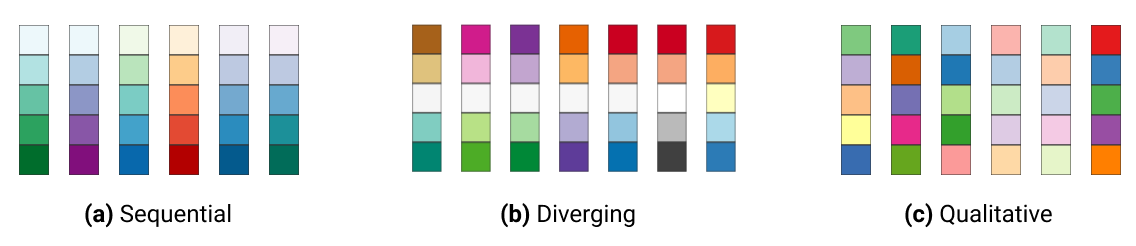
\includegraphics[width=\textwidth, height=0.22\textheight, keepaspectratio]{images/fig_7_6_color_palettes.png}\\[0.1cm]
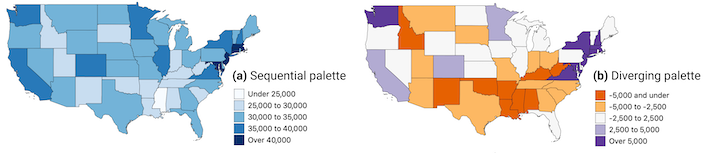
\includegraphics[width=\textwidth, height=0.26\textheight, keepaspectratio]{images/fig_7_7_sequential_vs_diverging.png}\\[0.1cm]
{\fontsize{6.5pt}{7.8pt}\selectfont \textcolor{navyMuted}{\textit{Hình 7.6: 3 hệ màu ColorBrewer \& Hình 7.7: Tuần tự vs Phân kỳ thu nhập Mỹ.}}}
\end{column}
\end{columns}
\slidenumber{13}
\end{frame}

% ==================== SLIDE 14: PHÂN KHOẢNG MÀU: STEPS VS CONTINUOUS ====================


\begin{frame}[plain, t]


\slideheader{Mục 03 • Thiết Kế Choropleth}{Phân Khoảng Màu: Bậc Thang (Steps) vs. Liên Tục}
\begin{columns}[T]
\begin{column}{0.52\textwidth}
{\fontsize{7.8pt}{9.8pt}\selectfont
\begin{table}[h]
\centering
\begin{tabular}{p{0.45\textwidth} p{0.45\textwidth}}
\toprule
\textbf{\color{navyMain} Bậc thang (Steps / Classes)} & \textbf{\color{navyMain} Dải màu liên tục (Continuous)} \\
\midrule
Chia thành $3\text{--}7$ ô màu rời rạc như bậc cầu thang. & Chuyển màu mượt mà không có vạch ngăn cách. \\
\midrule
\textbf{Ưu điểm:} Lý tưởng khi cần chỉ rõ vùng nằm trên/dưới một ngưỡng (VD: ngập lụt $>1\text{m}$). Dễ đối chiếu Chú giải (Legend). & \textbf{Ưu điểm:} Phản ánh khác biệt tinh tế (\textit{subtle nuances}). Tránh việc 2 vùng sát giá trị nhau bị đẩy sang 2 màu khác biệt. \\
\midrule
\textit{Lưu ý:} Quá nhiều bậc ($>7$) mắt không phân biệt nổi sắc độ kế cận. & \textit{Lưu ý:} Cần thuật toán nội suy phù hợp để không chìm màu ở khoảng giữa. \\
\bottomrule
\end{tabular}
\end{table}
}
\end{column}
\begin{column}{0.44\textwidth}
\centering
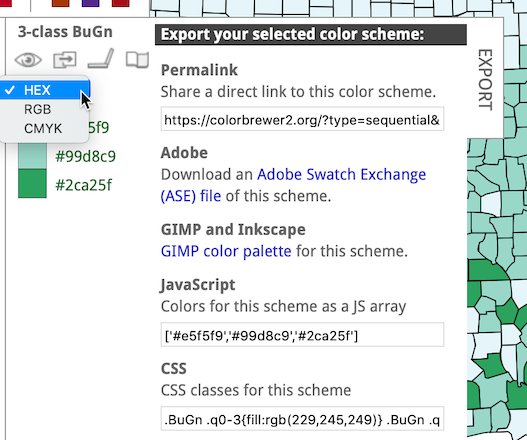
\includegraphics[width=\textwidth, height=0.52\textheight, keepaspectratio]{images/fig_7_9_steps_vs_continuous.png}\\[0.15cm]
{\fontsize{6.8pt}{8pt}\selectfont \textcolor{navyMuted}{\textit{Hình 7.9: Phân khoảng Bậc thang Steps (trái) vs Dải màu Liên tục (phải).}}}
\end{column}
\end{columns}
\slidenumber{14}
\end{frame}

% ==================== SLIDE 15: 3 PHƯƠNG PHÁP NỘI SUY (INTERPOLATION) ====================


\begin{frame}[plain, t]


\slideheader{Mục 03 • Thiết Kế Choropleth}{3 Phương Pháp Nội Suy Chia Nhóm Dữ Liệu}
\begin{columns}[T]
\begin{column}{0.52\textwidth}
{\fontsize{8.2pt}{10.5pt}\selectfont
\textbf{Luôn vẽ Histogram trước} để xem phân bố đối xứng hay lệch đuôi:

\vspace{0.12cm}
\textbf{1. Tuyến tính (Linear / Equal Interval):}
\begin{itemize}\setlength{\itemsep}{1.5pt}
    \item Chia đều khoảng cách min--max. Dành cho dữ liệu \textbf{phân bố chuẩn đối xứng}, làm nổi bật điểm cực đoan (outliers).
\end{itemize}

\textbf{2. Phân vị (Quantiles -- Quartiles, Quintiles):}
\begin{itemize}\setlength{\itemsep}{1.5pt}
    \item Mỗi nhóm màu chứa \textbf{số lượng đơn vị bằng nhau}. Phù hợp dữ liệu \textbf{bị lệch nặng (skewed)}, tận dụng tối đa dải màu.
\end{itemize}

\textbf{3. Điểm gãy tự nhiên (Jenks Natural Breaks):}
\begin{itemize}\setlength{\itemsep}{1.5pt}
    \item Gom giá trị gần nhau, tối đa hóa khoảng cách giữa các nhóm. \textbf{Thỏa hiệp cân bằng hoàn hảo} trên dữ liệu thực tế.
\end{itemize}
}
\end{column}
\begin{column}{0.44\textwidth}
\centering
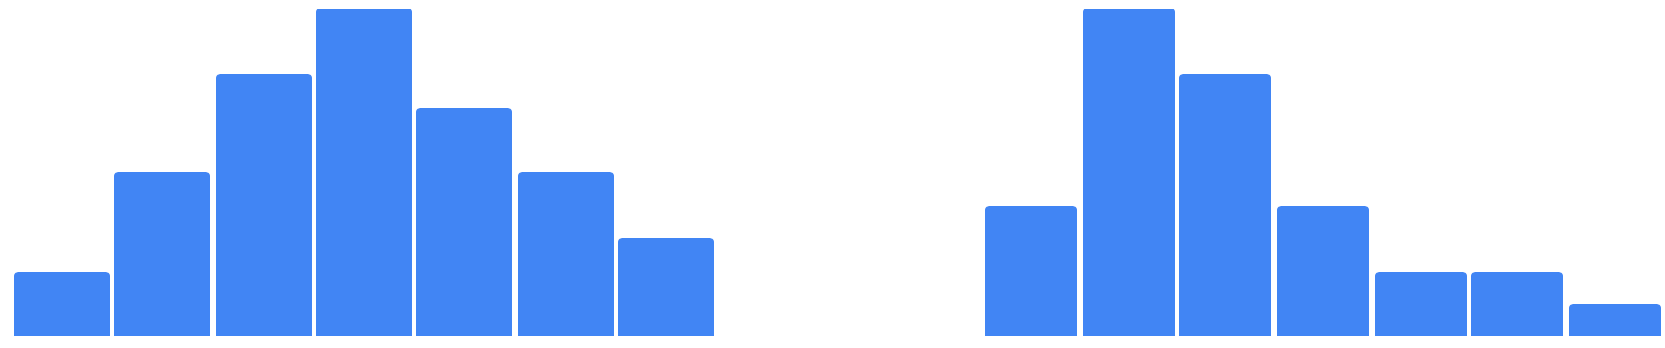
\includegraphics[width=\textwidth, height=0.22\textheight, keepaspectratio]{images/fig_7_12_histograms.png}\\[0.1cm]
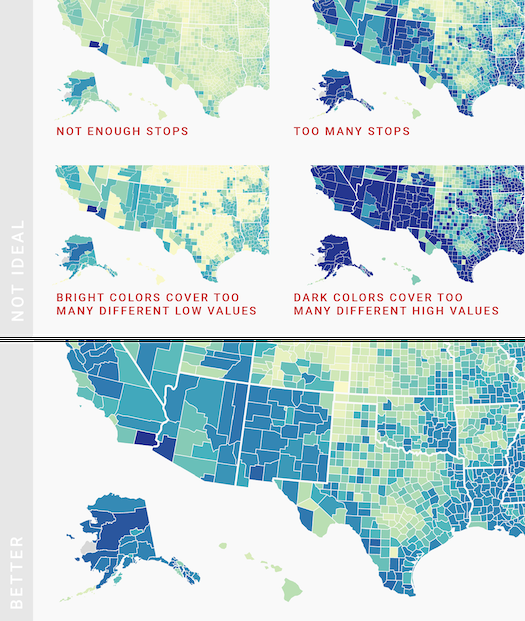
\includegraphics[width=\textwidth, height=0.26\textheight, keepaspectratio]{images/fig_7_13_full_color_range.png}\\[0.1cm]
{\fontsize{6.5pt}{7.8pt}\selectfont \textcolor{navyMuted}{\textit{Hình 7.12: Histogram phân bố lệch \& Hình 7.13: Tận dụng toàn dải màu.}}}
\end{column}
\end{columns}
\slidenumber{15}
\end{frame}

% ==================== SLIDE 16: QUY TẮC SỐNG CÒN: BẮT BUỘC CHUẨN HÓA ====================


\begin{frame}[plain, t]


\slideheader{Mục 03 • Thiết Kế Choropleth}{Quy Tắc Sống Còn: Bắt Buộc Chuẩn Hóa Bản Đồ!}
\calloutbox[\textwidth]{Cảnh Báo Kinh Điển: Bẫy Bản Đồ Mật Độ Dân Số}{
    Nếu đưa thẳng \textbf{số đếm thô (raw counts)} lên bản đồ Choropleth, bạn sẽ vô tình vẽ lại một \textbf{bản đồ mật độ dân số} hoàn toàn vô nghĩa thay vì hiện tượng nghiên cứu!
}

\begin{columns}[T]
\begin{column}{0.52\textwidth}
{\fontsize{7.8pt}{9.8pt}\selectfont
\textbf{Case Study Covid-19 tại Mỹ (26/06/2020 -- NYT):}
\begin{itemize}\setlength{\itemsep}{1.5pt}
    \item \textbf{(a) Tổng ca thô:} California, Texas, Florida đậm nhất $\rightarrow$ \textcolor{accentRed}{\textbf{Sai lầm}} vì đây đơn giản là các bang đông dân nhất!
    \item \textbf{(b) Ca trên đầu người (Per Capita):} $\frac{\text{Số ca}}{\text{Dân số}}$.
    \item \textbf{Sự thật lộ diện:} California \& Texas tỷ lệ rất thấp; tâm dịch thực sự tập trung dày đặc ở \textbf{New York, New Jersey, Massachusetts} và vùng \textbf{Louisiana}!
\end{itemize}
}
\end{column}
\begin{column}{0.44\textwidth}
\centering
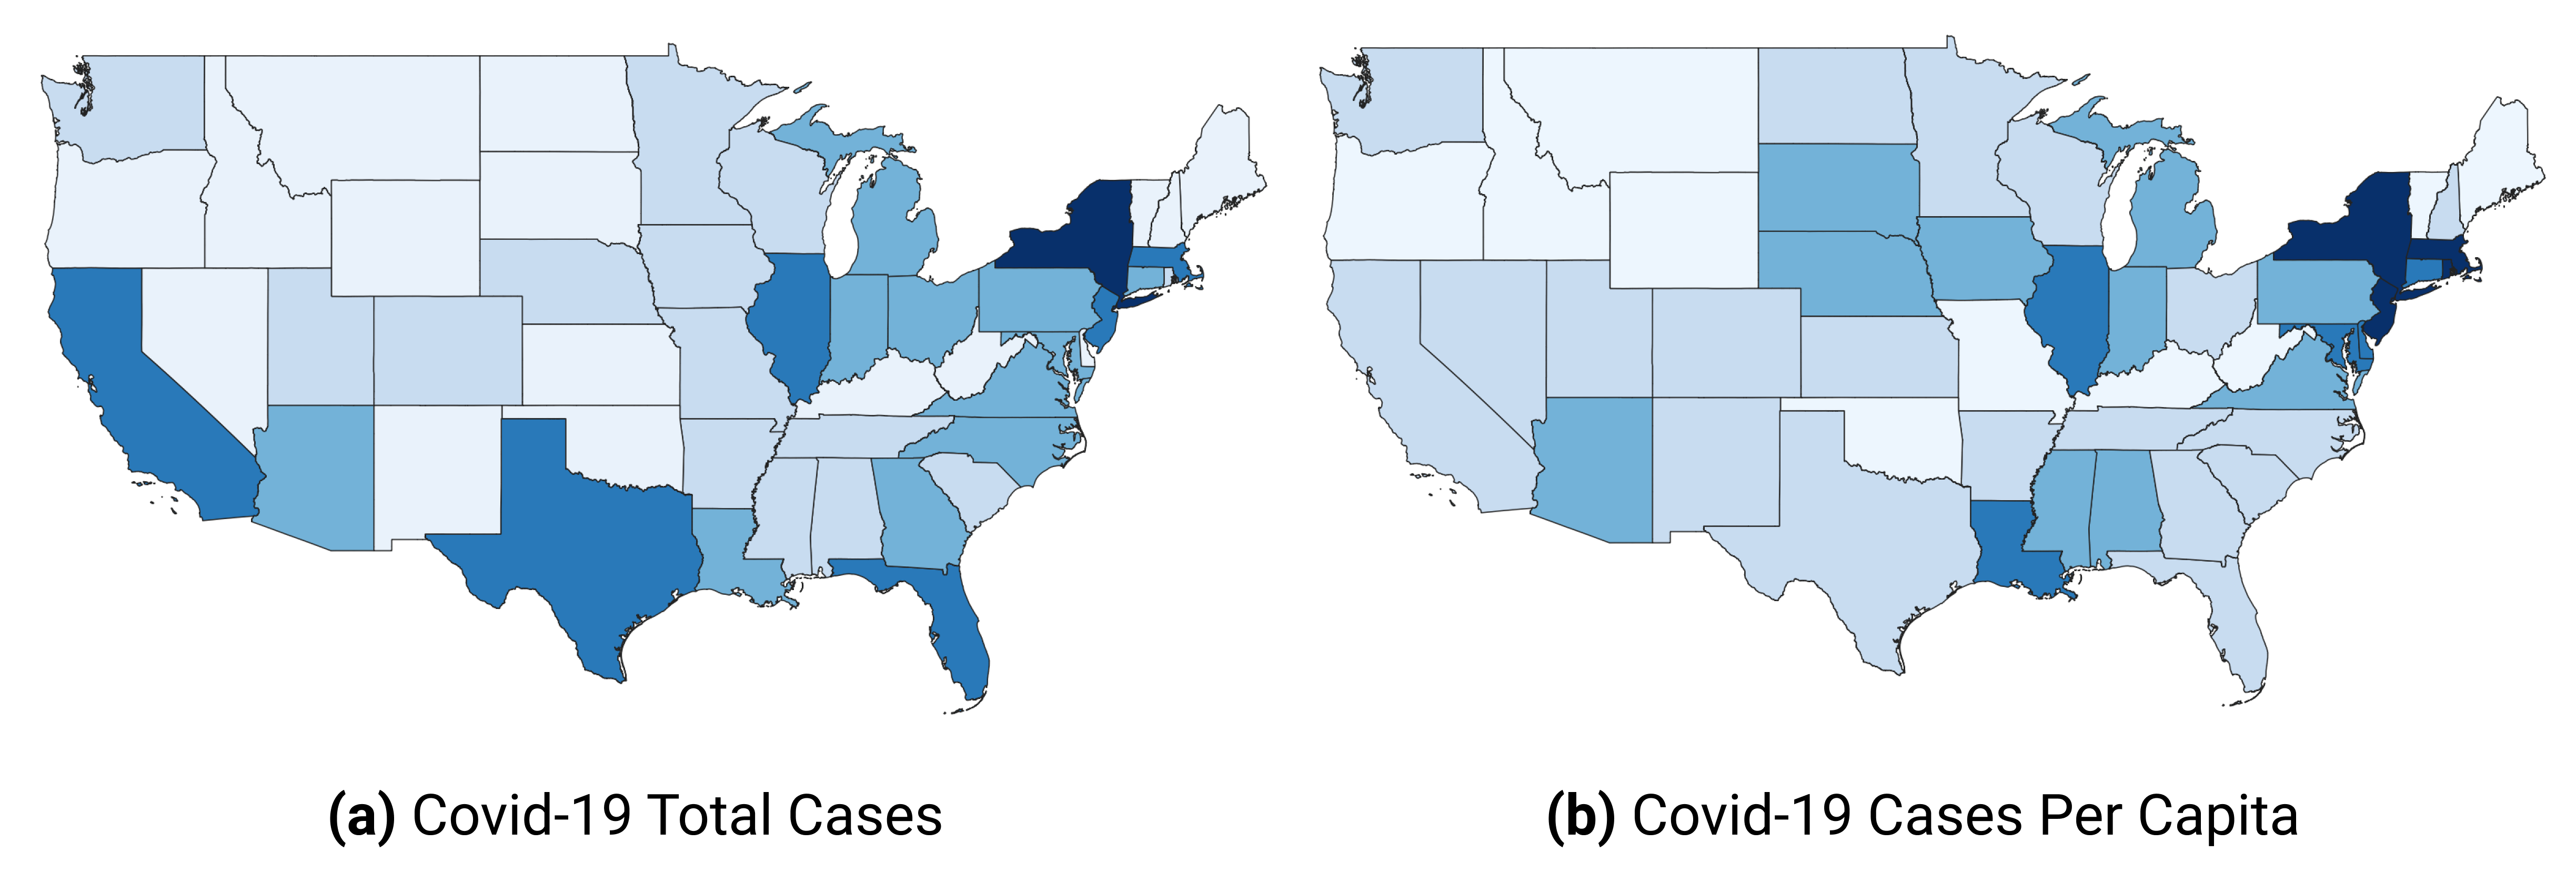
\includegraphics[width=\textwidth, height=0.48\textheight, keepaspectratio]{images/fig_7_14_normalize_covid_map.png}\\[0.12cm]
{\fontsize{6.8pt}{8pt}\selectfont \textcolor{navyMuted}{\textit{Hình 7.14: (a) Tổng ca thô gây hiểu lầm vs (b) Ca trên đầu người chính xác.}}}
\end{column}
\end{columns}
\slidenumber{16}
\end{frame}

% ==================== SLIDE 17: BẢN ĐỒ THỜI GIAN THỰC & BẪY NULL ISLAND ====================


\begin{frame}[plain, t]


\slideheader{Mục 03 • Thiết Kế Choropleth}{Bản Đồ Thời Gian Thực \& Bài Học Lọc Không Gian}
\begin{columns}[T]
\begin{column}{0.52\textwidth}
{\fontsize{8.2pt}{10.5pt}\selectfont
\textbf{Case Study: Bản đồ tai nạn chết người tại NYC (Socrata)}
Để bản đồ tự cập nhật dữ liệu mở chính xác, cần 3 bộ lọc:
\begin{enumerate}\setlength{\itemsep}{1.5pt}
    \item \textbf{Mức nghiêm trọng:} \texttt{PERSONS KILLED > 0}.
    \item \textbf{Thời gian cuốn chiếu:} \texttt{CRASH DATE = Last 365 days}.
    \item \textbf{Lọc lỗi tọa độ Null Island (0,0):} Rất nhiều vụ tai nạn chưa rõ vị trí bị gán về tọa độ $(0, 0)$ ngoài biển $\rightarrow$ Bắt buộc lọc \textbf{\texttt{LATITUDE > 0}} để giữ lại khu vực New York!
\end{enumerate}

\vspace{0.12cm}
\textbf{Rủi ro phụ thuộc bên thứ ba:}
Nếu cơ quan công quyền đổi tên cột hoặc ngắt API, bản đồ nhúng web sẽ lập tức bị hỏng.
}
\end{column}
\begin{column}{0.44\textwidth}
\centering
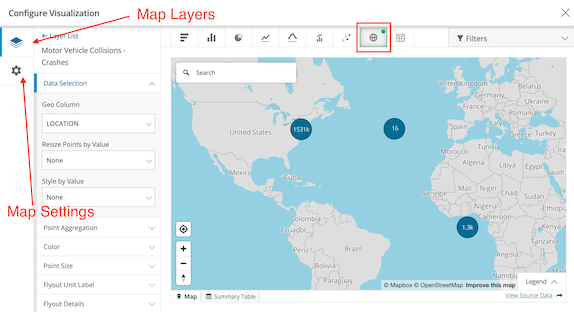
\includegraphics[width=\textwidth, height=0.22\textheight, keepaspectratio]{images/fig_7_63_null_island_crash.png}\\[0.1cm]
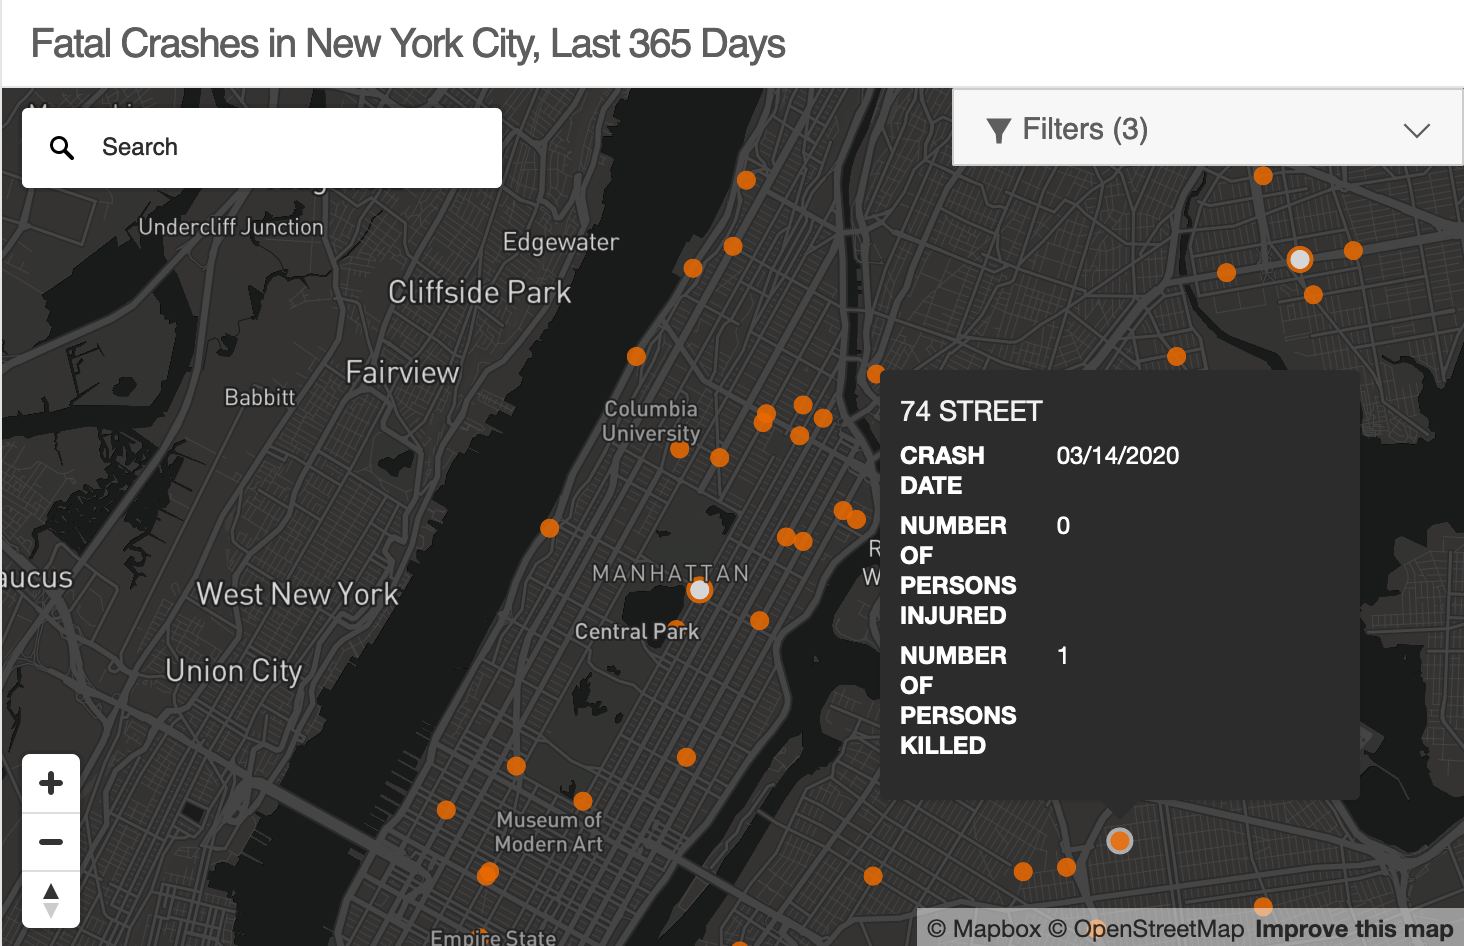
\includegraphics[width=\textwidth, height=0.25\textheight, keepaspectratio]{images/fig_7_61_nyc_crashes.png}\\[0.1cm]
{\fontsize{6.5pt}{7.8pt}\selectfont \textcolor{navyMuted}{\textit{Hình 7.63: Lỗi văng điểm ra Null Island \& Hình 7.61: Bản đồ sau khi lọc sạch.}}}
\end{column}
\end{columns}
\slidenumber{17}
\end{frame}

% ==================== SLIDE 18: TỔNG KẾT PHẦN 3 ====================


\begin{frame}[plain, t]


\slideheader{Phần 3 • Tổng Kết}{Nguyên Tắc Vàng Khi Trực Quan Hóa Không Gian}
\begin{columns}[T]
\begin{column}{0.31\textwidth}
\begin{tikzpicture}
    \node[draw=navyMain, fill=boxBg, rounded corners=6pt, line width=0.9pt, inner sep=7pt, text width=\textwidth-16pt, align=left] {
        {\fontsize{9pt}{11pt}\selectfont \textbf{\color{navyMain} 1. ĐÚNG HÌNH THÁI}}\\[0.05cm]
        {\fontsize{7.5pt}{9.2pt}\selectfont \color{navyMuted} Lựa chọn khôn ngoan}\\[0.12cm]
        {\fontsize{7.2pt}{9pt}\selectfont \color{navyMain}
        • Chỉ vẽ bản đồ khi yếu tố địa lý mang lại quy luật mới\\
        • Ưu tiên nền Vector sắc nét\\
        • Phân biệt Point vs Polygon\\
        • Linh hoạt gộp Điểm vào Vùng}
    };
\end{tikzpicture}
\end{column}
\begin{column}{0.31\textwidth}
\begin{tikzpicture}
    \node[draw=navyMain, fill=boxBg, rounded corners=6pt, line width=0.9pt, inner sep=7pt, text width=\textwidth-16pt, align=left] {
        {\fontsize{9pt}{11pt}\selectfont \textbf{\color{navyMain} 2. ĐƠN GIẢN \& CHI TIẾT}}\\[0.05cm]
        {\fontsize{7.5pt}{9.2pt}\selectfont \color{navyMuted} Nguyên tắc thiết kế}\\[0.12cm]
        {\fontsize{7.2pt}{9pt}\selectfont \color{navyMain}
        • Chỉ 1 biến trên bản đồ, tránh quá tải khi chồng 2 biến\\
        • Dùng Scatter Chart cho 2 biến\\
        • Chọn đơn vị địa lý nhỏ hơn (cấp Hạt thay vì cấp Bang)\\
        • Khắc phục bài toán MAUP}
    };
\end{tikzpicture}
\end{column}
\begin{column}{0.31\textwidth}
\begin{tikzpicture}
    \node[draw=navyMain, fill=boxBg, rounded corners=6pt, line width=0.9pt, inner sep=7pt, text width=\textwidth-16pt, align=left] {
        {\fontsize{9pt}{11pt}\selectfont \textbf{\color{navyMain} 3. CHOROPLETH CHUẨN}}\\[0.05cm]
        {\fontsize{7.5pt}{9.2pt}\selectfont \color{navyMuted} Màu sắc \& Chuẩn hóa}\\[0.12cm]
        {\fontsize{7.2pt}{9pt}\selectfont \color{navyMain}
        • Bảng màu ColorBrewer chuẩn\\
        • Xem Histogram trước khi chọn Linear, Quantile, Jenks\\
        • \textbf{Bắt buộc chuẩn hóa} số thô sang tỷ lệ Per Capita\\
        • Lọc sạch lỗi Null Island}
    };
\end{tikzpicture}
\end{column}
\end{columns}
\vspace{0.3cm}
\centering
\pillbox{\fontsize{9pt}{11pt}\selectfont Tiếp theo: Phần 4 -- Đạo Đức Dữ Liệu \& Nghệ Thuật Kể Chuyện (Chương 14 \& 15)}
\slidenumber{18}
\end{frame}

% ==================== SLIDE 1: TIÊU ĐỀ PHẦN 4 ====================


\end{document}
